\documentclass[8pt,a4paper,landscape]{extarticle}
\makeatletter
\def\input@path{{../_shared/}}
\makeatother
\usepackage{cheatsheet}
\usepackage{graphicx}

\begin{document}
\begin{multicols*}{4}

\cheattitle{Computer Systems}{}{BA4}

\begin{warn}[title=]
    \begin{tabular}{ll}
    \textbf{Protocols / Technologies} & \textbf{Layer} \\
    \hline
    HTTP, DNS, BitTorrent & Application \\
    TCP, UDP              & Transport \\
    IP                    & Network \\
    WiFi, Ethernet, FTTH  & Link \\
    EM waves, optical, electric & Physical \\
    \end{tabular}
\end{warn}

\section{Lecture 8 - Forwarding and IP}

\begin{prop}[title=Headers]
\begin{itemize}
    \item \textbf{Transport header - TCP}: SYN flag, checksum, SEQ, ACK, receiver window, src/dst port.
    \item \textbf{Network header - IP:} src/dst IP addr. 
\end{itemize}
\end{prop}

\subsection{Network Layer functions}

\subsubsection{Forwarding}
\begin{defn}[title=Forwarding]
Determines the output link for each packet.
\textbf{How:} \textbf{read} field from packet's network layer header, \textbf{search} forwarding table for output link.
\end{defn}

\subsubsection{Routing}
\begin{defn}[title=Routing]
Populates forwarding tables.
\textbf{How:} routing algorithm run on a logically centralised \textbf{network controller} or the \textbf{routers themselves}
\end{defn}

\subsection{Internet (IP) forwarding}
{\centering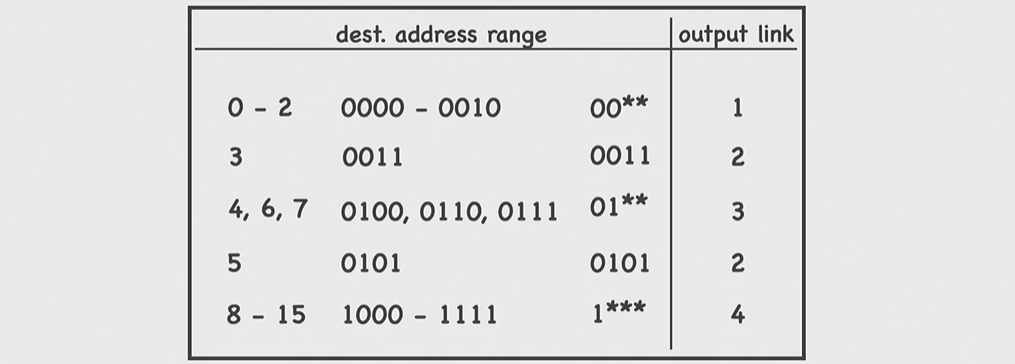
\includegraphics[width=\linewidth,height=2.8cm,keepaspectratio]{images/lecture08/forwarding-table.png}\par}
Each entry is a \textbf{prefix} (e.g.\ \texttt{01**}); a packet is forwarded using the \textbf{longest matching prefix}.

\begin{defn}[title=IP prefix]
\texttt{a.b.c.d/n} denotes a range of addresses sharing the same first $n$ bits (prefix length); the remaining $32-n$ bits are wildcards.
\end{defn}

\subsubsection{IP subnet (subnetwork)}
{\centering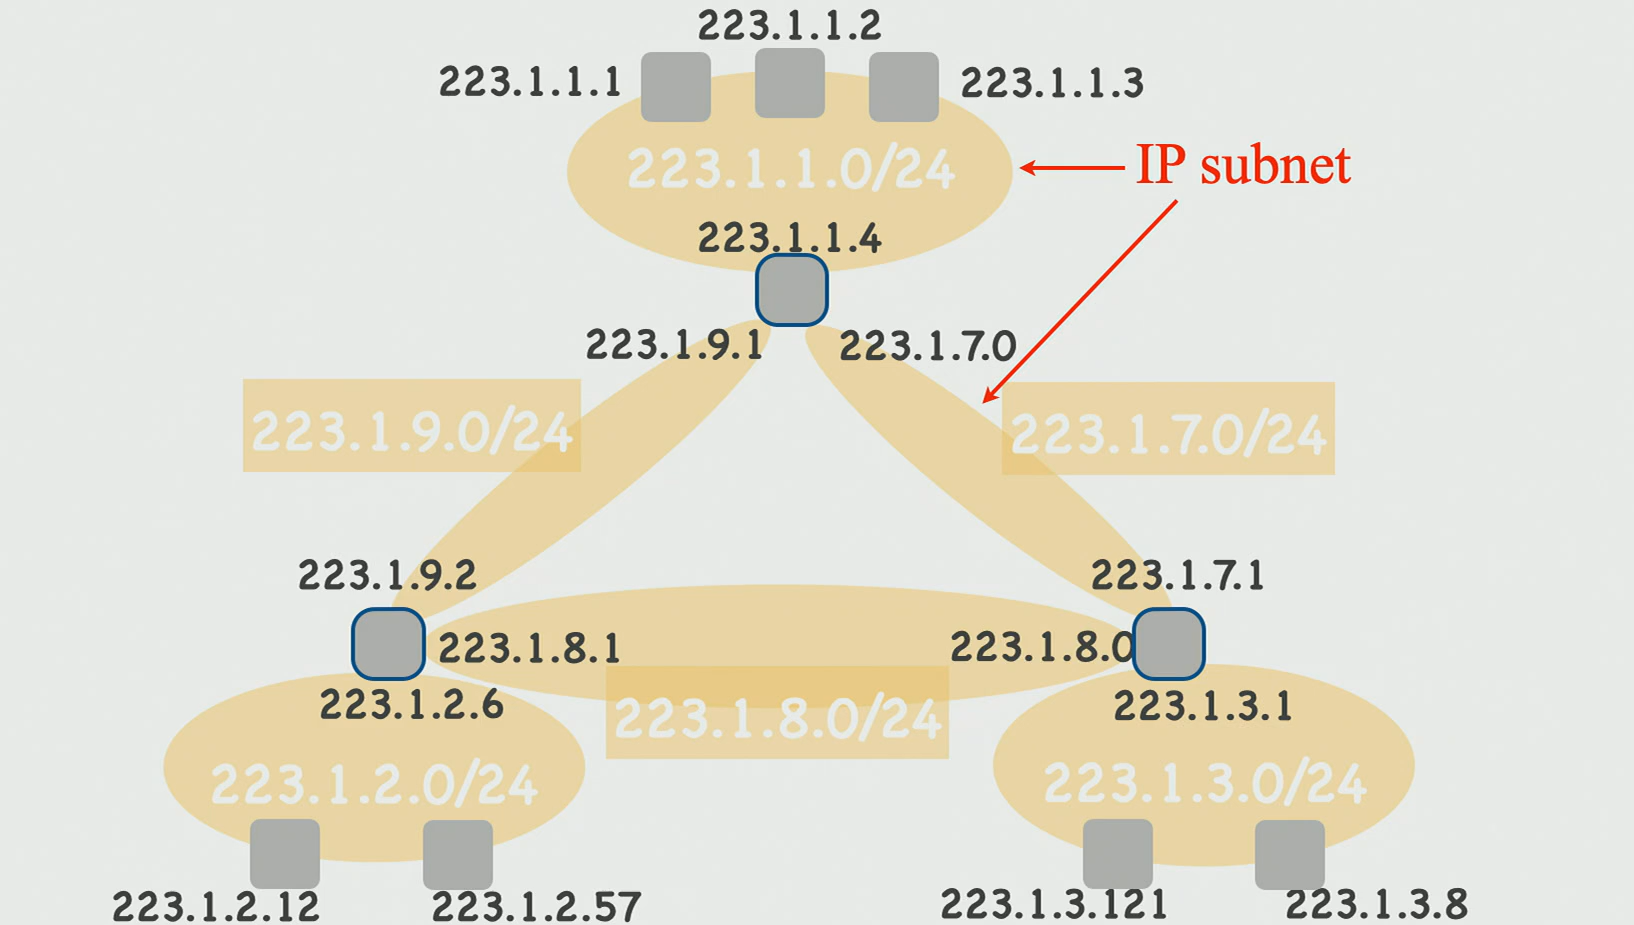
\includegraphics[width=\linewidth,height=2.8cm,keepaspectratio]{images/lecture08/ip-subnet-overview.png}\par}

\begin{defn}[title=Broadcast IP address]
The \texttt{biggest IP address} an IP subnet. If a packet has this destination, it's destined to \textbf{all the end-systems} and \textbf{routers} in the IP subnet.
\end{defn}

\begin{prop}[title=Internet principle]
    \textbf{Global reachability:} Every end-system must be reachable from any other end-system.
\end{prop}
 
\subsection{Network Address Translation (NAT)}

\begin{defn}[title=Definition]
    A router becomes a NAT only when it's configured to translate between private and public addresses.
\end{defn}

\begin{prop}[title=How does it work]
    \begin{itemize}
        \item Resolves IP address depletion problem
        \item Rewrites src IP add. and port \# of outg. packets
        \item Rewrites dst IP add. and port \# of inc. packets
    \end{itemize}
\end{prop}

\begin{thm}[title=Layering violation (but it works)]
    \begin{itemize}
        \item Requires \textbf{per-connection state} at the border routers of the private IP subnets.
        \item An end-system inside a private IP subnet is \textbf{unreachable} from the outside world. [trick possible]
    \end{itemize}
\end{thm}

\subsubsection{NAT example}
{\centering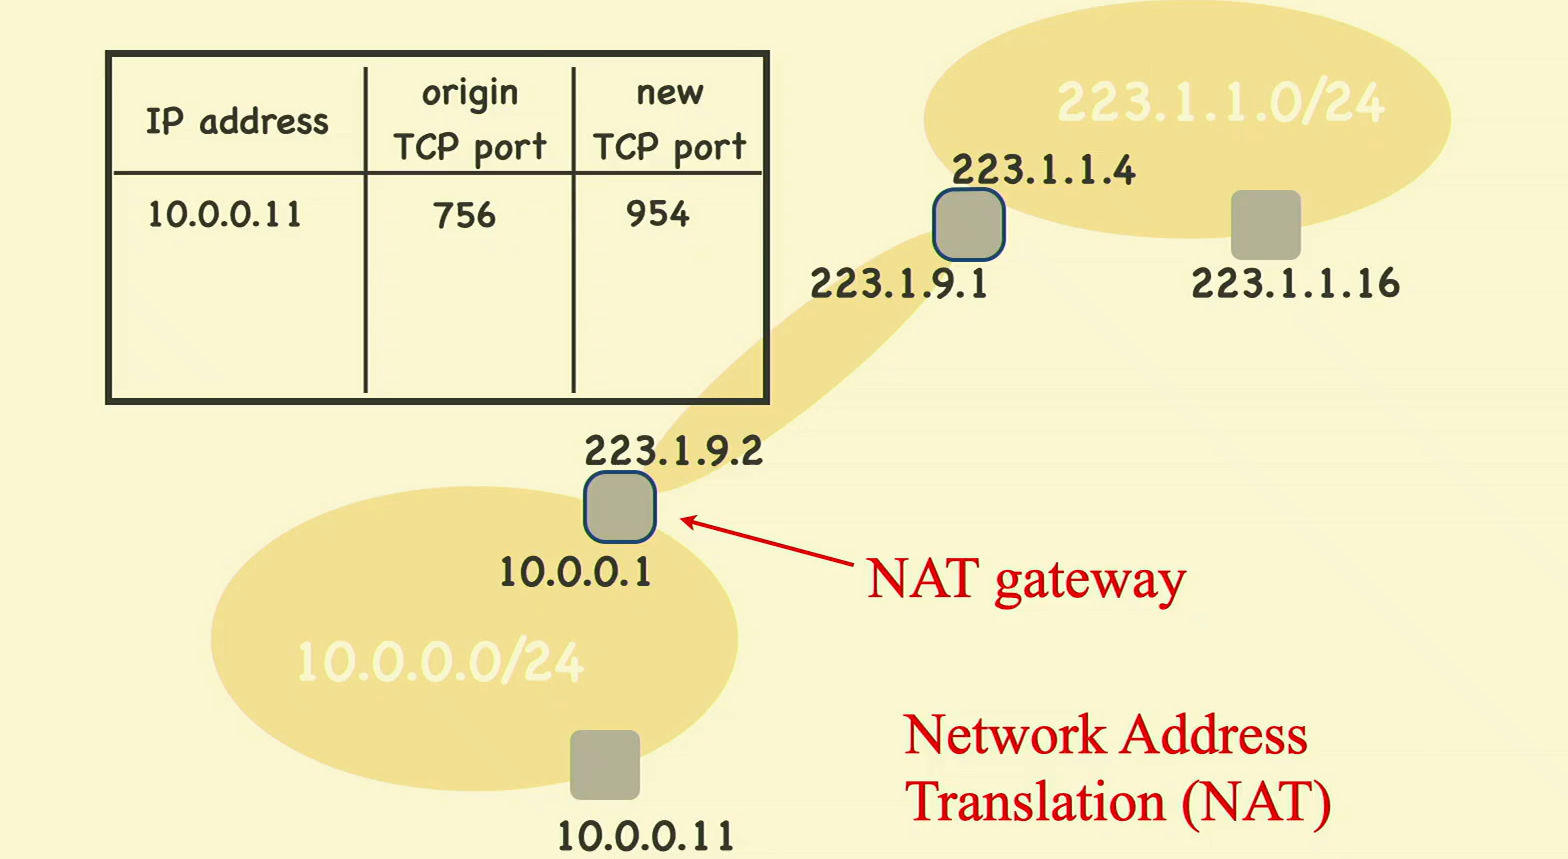
\includegraphics[width=\linewidth,height=2.8cm,keepaspectratio]{images/lecture08/nat-overview.png}\par}

\section{Lecture 9 - Routing \& BGP}

\begin{defn}[title=First-hop router]
    First router packets hit when leaving a subnet.
\end{defn}

\subsection{Internet Routing algorithms}

\begin{prop}[title=Dijkstra's (Link state routing algo)]
    \begin{enumerate}
        \item At each step, consider a new router starting from "closest" neighbor
        \item Check whether current paths can be improved
        \item End when no improvement is possible
    \end{enumerate}
\end{prop}
\begin{prop}[title=Bellman-Ford (Distance vector)]
    \begin{enumerate}
        \item All neighbors exchange information
        \item Each router checks whether it can improve current paths by leveraging the new information
        \item End when no improvement is possible
    \end{enumerate}
\end{prop}

\begin{warn}[title=Link state VS Distance vector]
    \begin{itemize}
        \item Link state converges faster
        \item Distance vector uses less bandwitdh
    \end{itemize}
\end{warn}

\subsection{Putting things together}

\subsubsection{}

\begin{thm}[title=Internet rounting challenges]
    \begin{itemize}
        \item \textbf{Admin:} An ISP may want to hide its link costs
        \item \textbf{Scale:} Too many IP subnets may cause trouble
    \end{itemize}
\end{thm}

\begin{defn}[title=Autonomous System (AS)]
    A network or group of networks under a \textbf{single administrative authority}, running its own internal routing protocol. Identified by a unique \textbf{ASN}.
\end{defn}

\subsection{Inter-AS Routing (BGP)}
Routing \textbf{between} ASes. One universal protocol based on Bellman-Ford. Not always the shortest path.

\begin{prop}[title=Border Gateway Protocol (BGP)]
    \begin{enumerate}
        \item All neighbors exchange reachable prefixes
        \item Each router checks whether it can improve paths
        \item End when no improvement is possible
    \end{enumerate}
\end{prop}

\begin{thm}[title=Internet rounting solutions]
    \begin{itemize}
        \item Router $\leftrightarrow$ with \textbf{local} router
        \item Border router $\leftrightarrow$ with \textbf{external neighbor}
        \item Router keeps \textbf{forwarding state} for (1) \textbf{local IP subnets} and (2) \textbf{foreign aggregate IP prefixe}
    \end{itemize}
\end{thm}

% Concrètement: Je ne connais pas toutes les maisons du monde. Je sais seulement sur quelle île aller. Une fois sur l'île, les habitants connaissent les routes locales et me dirigent vers la bonne maison.

\section{Lecture 10 - Link layer \& Ethernet}

\begin{defn}[title=Recall: Packet Switches types]
    \begin{itemize}
        \item \textbf{Network layer:} L3 = \underline{Routers}
        \item \textbf{Link layer}: L2 = \underline{Switches}. Ex: ethernet
    \end{itemize}
\end{defn}

\begin{prop}[title=Link layer services]
    \begin{itemize}
        \item Error detection \& Reliable data delivery
        \item \textit{Medium access control (MAC)}
    \end{itemize}
\end{prop}

\begin{defn}[title=Link layer header: MAC address]
48-bit. Flat: not location dependent
\end{defn}
{\centering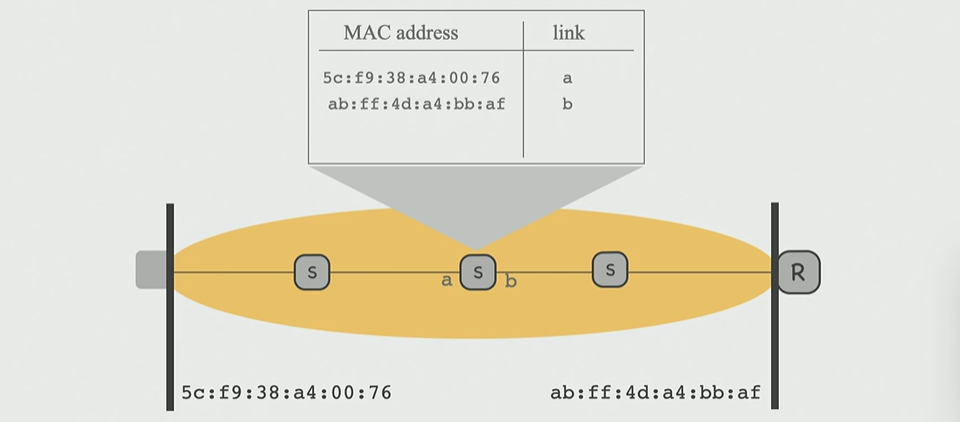
\includegraphics[width=\linewidth,height=2.8cm,keepaspectratio]{images/lecture10/L2-forwarding.png}\par}

\begin{prop}[title=Not a real routing]
Learn from traffic. Broadcast when unknown.
\end{prop}

\begin{thm}[title=Spanning tree Broadcast]
The naïve broadcast may lead to forwarding loops. Use spanning tree to avoid cycles.
\end{thm}

\begin{prop}[title=Address Resolution Protocol (ARP)]
\textbf{Goal:} Map IP addr. to MAC addr.\\
\textbf{How:} Broadcast + caching. 
\end{prop}

\begin{prop}[title=ARP vs DNS]
    \begin{itemize}
        \item \textbf{ARP:} Relies on broadcasting
        \item \textbf{DNS:} Relies on DNS structure
    \end{itemize}
\end{prop}

\begin{prop}[title=Three network levels]
    \begin{itemize}
        \item \textbf{IP Subnet:} L2 forwarding, L2 learning
        \item \textbf{AS:} IP (L3) forwarding, intra domain routing
        \item \textbf{Internet:} IP (L3) forwarding, BGP routing
    \end{itemize}
\end{prop}

\section{Lecture 12 - Processes and Threads}

\begin{defn}[title=Process]
    An instance of a running program. Has its own \textbf{isolated memory space} (code, data, heap, stack) and OS resources (file descriptors, etc.).
\end{defn}

\begin{defn}[title=Thread]
    A unit of execution \textbf{within} a process. Threads share the process's memory and resources, but each has its own \textbf{stack} and \textbf{program counter}.
\end{defn}

\begin{defn}[title=OS Scheduler]
    Allows each thread to run by allocating CPU time slices, switching between threads (context switch) to give the illusion of parallelism.
\end{defn}

\begin{prop}[title=Key properties]
    \begin{itemize}
        \item \textbf{Identifier}: unique id for processes and threads
        \item Each Thread/Process has the \textbf{illusion} that is it the only one occupying the CPU/Memory (resp.)
    \end{itemize}
\end{prop}

\section{Lecture 13 - Sharing the CPU}

\begin{defn}[title=Limited direct execution]
    A thread cannot do whatever it wants for as long as it wants. The CPU executes the thread's instructions without any intermediary.    
\end{defn}

\begin{prop}[title=CPU priviledge level = CPU mode]
    A state stored in the CPU. Either "low" or "high".
\end{prop}

\begin{prop}[title=CPU instructions]
    \begin{itemize}
        \item \textbf{Non-priviledged:} can be executed anytime
        \item \textbf{Priviledged:} only if it is in high mode
    \end{itemize}
\end{prop}

\begin{defn}[title=Kernel definition]
It is the software that runs with full privileges and manages the hardware on behalf of programs.
\end{defn}

\begin{prop}[title=User/Kernel mode]
    \begin{itemize}
        \item \textbf{Kernel mode:} High privilege
        \item \textbf{User mode:} Low privilege
    \end{itemize}
\end{prop}

\begin{thm}[title=3 mechanisms to invoke the kernel]
    Syscall ; Exception/Trap ; Interrupt
\end{thm}

{\centering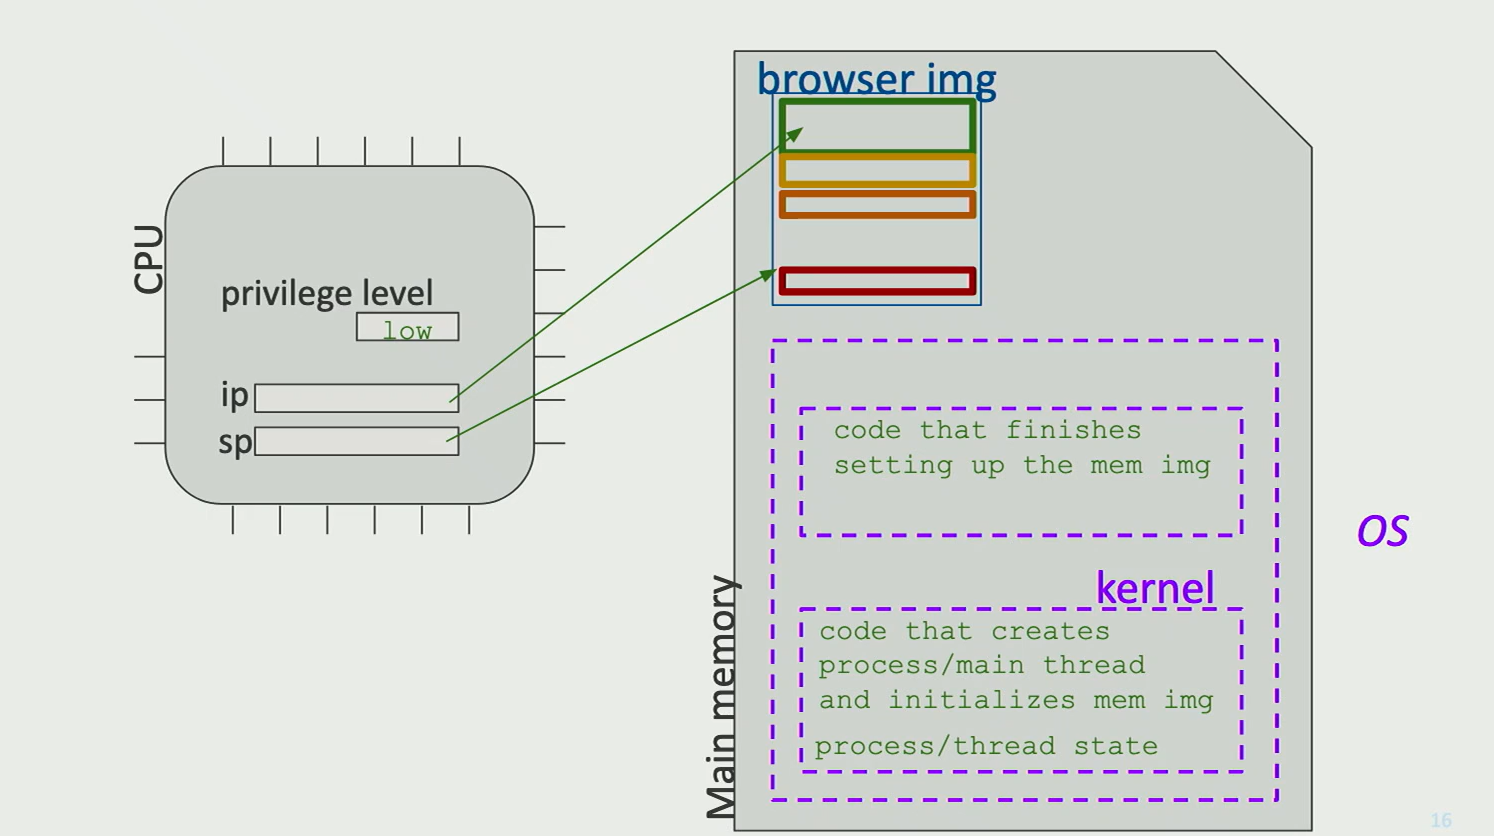
\includegraphics[width=\linewidth,height=2.8cm,keepaspectratio]{images/lecture13/kernel_overview.png}\par}

How threads can share the CPU \textbf{safely} and \textbf{fairly}?
\begin{thm}[title=Limited direct execution]
    \begin{itemize}
        \item A normal thread wants to do something high privilege $\rightarrow$ creates a syscall
        \item A thread tries to do something illegal $\rightarrow$ exception
        \item An externel entity needs attention $\rightarrow$ interrupt
    \end{itemize}
\end{thm}

How are processes created and destroyed?
\begin{prop}[title=Process lifecycle]
    \begin{itemize}
        \item \texttt{fork}: creates a \textbf{child} process (copy of parent)
        \item \texttt{exec}: replaces process image with a new program
        \item \texttt{exit}: terminates the process
        \item \texttt{wait}: parent waits for child to finish
    \end{itemize}
\end{prop}

\begin{prop}[title=Key processes]
    \begin{itemize}
        \item \textbf{Init}: first process after boot
        \item \textbf{Idle}: runs when nothing else can
        \item \textbf{Shell}: spawns new process on command
        \item \textbf{GUI manager}: spawns new process on click
    \end{itemize}
\end{prop}

\end{multicols*}
\end{document}
